\documentclass[12pt]{article}
\usepackage{fontspec}
\usepackage{fullpage}
\usepackage{hyperref}
\hypersetup{bookmarks=true,colorlinks=true,linkcolor=red,citecolor=blue,filecolor=magenta,urlcolor=cyan}
\usepackage{amsmath}
\usepackage{amssymb}
\usepackage{mathtools}
\usepackage{unicode-math}
\usepackage{tabularray}
\usepackage{tabularx}
\usepackage{booktabs}
\usepackage{caption}
\usepackage{graphics}
\usepackage{svg}
\usepackage{float}
\usepackage{enumitem}
\usepackage{adjustbox}
\usepackage{filecontents}
\usepackage[backend=bibtex]{biblatex}
\usepackage{url}
\setmathfont{Latin Modern Math}
\newcommand{\gt}{\ensuremath >}
\newcommand{\lt}{\ensuremath <}
\newlist{symbDescription}{description}{1}
\setlist[symbDescription]{noitemsep, topsep=0pt, parsep=0pt, partopsep=0pt}
\newcommand{\resizeExpression}[1]{
  \adjustbox{max width=\linewidth}{$#1$}
}
\bibliography{bibfile}
\title{Software Requirements Specification for Double Pendulum}
\author{Dong Chen}
\begin{document}
\maketitle
\tableofcontents
\newpage
\section{Reference Material}
\label{Sec:RefMat}
This section records information for easy reference.

\subsection{Table of Units}
\label{Sec:ToU}
The unit system used throughout is SI (Système International d'Unités). In addition to the basic units, several derived units are also used. For each unit, the \hyperref[Table:ToU]{Table of Units} lists the symbol, a description, and the SI name.

\begin{longtblr}
[caption={Table of Units}]
{colspec={l l l}, rowhead=1, hline{1,Z}=\heavyrulewidth, hline{2}=\lightrulewidth}
\textbf{Symbol} & \textbf{Description} & \textbf{SI Name}
\\
${\text{kg}}$ & mass & kilogram
\\
${\text{m}}$ & length & metre
\\
${\text{N}}$ & force & newton
\\
${\text{rad}}$ & angle & radian
\\
${\text{s}}$ & time & second
\label{Table:ToU}
\end{longtblr}
\subsection{Table of Symbols}
\label{Sec:ToS}
The symbols used in this document are summarized in the \hyperref[Table:ToS]{Table of Symbols} along with their units. Throughout the document, symbols in bold will represent vectors, and scalars otherwise. The symbols are listed in alphabetical order. For vector quantities, the units shown are for each component of the vector.

\begin{longtblr}
[caption={Table of Symbols}]
{colspec={l l l}, rowhead=1, hline{1,Z}=\heavyrulewidth, hline{2}=\lightrulewidth}
\textbf{Symbol} & \textbf{Description} & \textbf{Units}
\\
${a_{1}}$ & Acceleration of the first object & $\frac{\text{m}}{\text{s}^{2}}$
\\
${a_{2}}$ & Acceleration of the second object & $\frac{\text{m}}{\text{s}^{2}}$
\\
${a_{\text{x}1}}$ & Horizontal acceleration of the first object & $\frac{\text{m}}{\text{s}^{2}}$
\\
${a_{\text{x}2}}$ & Horizontal acceleration of the second object & $\frac{\text{m}}{\text{s}^{2}}$
\\
${a_{\text{y}1}}$ & Vertical acceleration of the first object & $\frac{\text{m}}{\text{s}^{2}}$
\\
${a_{\text{y}2}}$ & Vertical acceleration of the second object & $\frac{\text{m}}{\text{s}^{2}}$
\\
$\symbf{a}\text{(}t\text{)}$ & Acceleration & $\frac{\text{m}}{\text{s}^{2}}$
\\
$\symbf{F}$ & Force & ${\text{N}}$
\\
${f_{1}}$ & Force of the first object & ${\text{N}}$
\\
${f_{2}}$ & Force of the second object & ${\text{N}}$
\\
$g$ & Magnitude of gravitational acceleration & $\frac{\text{m}}{\text{s}^{2}}$
\\
$\symbf{g}$ & Gravitational acceleration & $\frac{\text{m}}{\text{s}^{2}}$
\\
$\symbf{\hat{i}}$ & Unit vector & --
\\
${L_{1}}$ & Length of the first rod & ${\text{m}}$
\\
${L_{2}}$ & Length of the second rod & ${\text{m}}$
\\
$m$ & Mass & ${\text{kg}}$
\\
${m_{1}}$ & Mass of the first object & ${\text{kg}}$
\\
${m_{2}}$ & Mass of the second object & ${\text{kg}}$
\\
${p_{\text{x}1}}$ & Horizontal position of the first object & ${\text{m}}$
\\
${p_{\text{x}2}}$ & Horizontal position of the second object & ${\text{m}}$
\\
${p_{\text{y}1}}$ & Vertical position of the first object & ${\text{m}}$
\\
${p_{\text{y}2}}$ & Vertical position of the second object & ${\text{m}}$
\\
$\symbf{p}\text{(}t\text{)}$ & Position & ${\text{m}}$
\\
$\symbf{T}$ & Tension & ${\text{N}}$
\\
${\symbf{T}_{1}}$ & Tension of the first rod & ${\text{N}}$
\\
${\symbf{T}_{2}}$ & Tension of the second rod & ${\text{N}}$
\\
$t$ & Time & ${\text{s}}$
\\
$\text{theta}$ & Dependent variables & ${\text{rad}}$
\\
${v_{1}}$ & Velocity of the first object & $\frac{\text{m}}{\text{s}}$
\\
${v_{2}}$ & Velocity of the second object & $\frac{\text{m}}{\text{s}}$
\\
${v_{\text{x}1}}$ & Horizontal velocity of the first object & $\frac{\text{m}}{\text{s}}$
\\
${v_{\text{x}2}}$ & Horizontal velocity of the second object & $\frac{\text{m}}{\text{s}}$
\\
${v_{\text{y}1}}$ & Vertical velocity of the first object & $\frac{\text{m}}{\text{s}}$
\\
${v_{\text{y}2}}$ & Vertical velocity of the second object & $\frac{\text{m}}{\text{s}}$
\\
$\symbf{v}\text{(}t\text{)}$ & Velocity & $\frac{\text{m}}{\text{s}}$
\\
${w_{1}}$ & Angular velocity of the first object & $\frac{\text{rad}}{\text{s}}$
\\
${w_{2}}$ & Angular velocity of the second object & $\frac{\text{rad}}{\text{s}}$
\\
${α_{1}}$ & Angular acceleration of the first object & $\frac{\text{rad}}{\text{s}^{2}}$
\\
${α_{2}}$ & Angular acceleration of the second object & $\frac{\text{rad}}{\text{s}^{2}}$
\\
${θ_{1}}$ & Angle of the first rod & ${\text{rad}}$
\\
${θ_{2}}$ & Angle of the second rod & ${\text{rad}}$
\\
$π$ & Ratio of circumference to diameter for any circle & --
\label{Table:ToS}
\end{longtblr}
\subsection{Abbreviations and Acronyms}
\label{Sec:TAbbAcc}
\begin{longtblr}
[caption={Abbreviations and Acronyms}]
{colspec={l l}, rowhead=1, hline{1,Z}=\heavyrulewidth, hline{2}=\lightrulewidth}
\textbf{Abbreviation} & \textbf{Full Form}
\\
2D & Two-Dimensional
\\
A & Assumption
\\
DD & Data Definition
\\
DblPend & Double Pendulum
\\
GD & General Definition
\\
GS & Goal Statement
\\
IM & Instance Model
\\
PS & Physical System Description
\\
R & Requirement
\\
RefBy & Referenced by
\\
Refname & Reference Name
\\
SRS & Software Requirements Specification
\\
TM & Theoretical Model
\\
Uncert. & Typical Uncertainty
\label{Table:TAbbAcc}
\end{longtblr}
\section{Introduction}
\label{Sec:Intro}
A pendulum consists of mass attached to the end of a rod and its moving curve is highly sensitive to initial conditions. Therefore, it is useful to have a program to simulate the motion of the pendulum to exhibit its chaotic characteristics. The document describes the program called Double Pendulum , which is based on the original, manually created version of \hyperref{https://github.com/Zhang-Zhi-ZZ/CAS741Project/tree/master/Double%20Pendulum}{}{}{Double Pendulum}.

The following section provides an overview of the Software Requirements Specification (SRS) for Double Pendulum. This section explains the purpose of this document, the scope of the requirements, the characteristics of the intended reader, and the organization of the document.

\subsection{Purpose of Document}
\label{Sec:DocPurpose}
The primary purpose of this document is to record the requirements of DblPend. Goals, assumptions, theoretical models, definitions, and other model derivation information are specified, allowing the reader to fully understand and verify the purpose and scientific basis of DblPend. With the exception of \hyperref[Sec:SysConstraints]{system constraints}, this SRS will remain abstract, describing what problem is being solved, but not how to solve it.

This document will be used as a starting point for subsequent development phases, including writing the design specification and the software verification and validation plan. The design document will show how the requirements are to be realized, including decisions on the numerical algorithms and programming environment. The verification and validation plan will show the steps that will be used to increase confidence in the software documentation and the implementation. Although the SRS fits in a series of documents that follow the so-called waterfall model, the actual development process is not constrained in any way. Even when the waterfall model is not followed, as Parnas and Clements point out \cite{parnasClements1986}, the most logical way to present the documentation is still to ``fake'' a rational design process.

\subsection{Scope of Requirements}
\label{Sec:ReqsScope}
The scope of the requirements includes the analysis of a two-dimensional (2D) pendulum motion problem with various initial conditions using Clifford algebra for geometric representation of physical quantities.

\subsection{Characteristics of Intended Reader}
\label{Sec:ReaderChars}
Reviewers of this documentation should have an understanding of undergraduate level 2 physics, undergraduate level 1 calculus, and ordinary differential equations. The users of DblPend can have a lower level of expertise, as explained in \hyperref[Sec:UserChars]{Sec:User Characteristics}.

\subsection{Organization of Document}
\label{Sec:DocOrg}
The organization of this document follows the template for an SRS for scientific computing software proposed by \cite{koothoor2013}, \cite{smithLai2005}, \cite{smithEtAl2007}, and \cite{smithKoothoor2016}. The presentation follows the standard pattern of presenting goals, theories, definitions, and assumptions. For readers that would like a more bottom up approach, they can start reading the \hyperref[Sec:IMs]{instance models} and trace back to find any additional information they require.

The \hyperref[Sec:GoalStmt]{goal statements} are refined to the theoretical models and the \hyperref[Sec:TMs]{theoretical models} to the \hyperref[Sec:IMs]{instance models}. This document demonstrates a novel approach to modeling the double pendulum using Clifford algebra. The traditional vector-based approach is enhanced by representing physical quantities as multivector in a unified geometric framework. Section 4.2.3 presents general definitions that showcase how velocity, acceleration, and force are naturally expressed using Clifford algebra operations such as the geometric product and basis vector representations..

\section{General System Description}
\label{Sec:GenSysDesc}
This section provides general information about the system. It identifies the interfaces between the system and its environment, describes the user characteristics, and lists the system constraints.

\subsection{System Context}
\label{Sec:SysContext}
\hyperref[Figure:sysCtxDiag]{Fig:sysCtxDiag} shows the system context. A circle represents an entity external to the software, the user in this case. A rectangle represents the software system itself (DblPend). Arrows are used to show the data flow between the system and its environment.

\begin{figure}[H]
\begin{center}
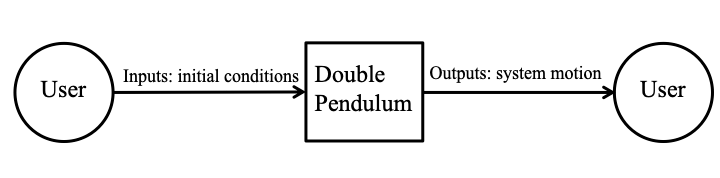
\includegraphics[width=\textwidth]{../../../../datafiles/dblpend/SystemContextFigure.png}
\caption{System Context}
\label{Figure:sysCtxDiag}
\end{center}
\end{figure}
The interaction between the product and the user is through an application programming interface. The responsibilities of the user and the system are as follows:

\begin{itemize}
\item{User Responsibilities}
\begin{itemize}
\item{Provide initial conditions of the physical state of the motion and the input data related to the Double Pendulum, ensuring no errors in the data entry.}
\item{Ensure that consistent units are used for input variables.}
\item{Ensure required \hyperref[Sec:Assumps]{software assumptions} are appropriate for any particular problem input to the software.}
\end{itemize}
\item{DblPend Responsibilities}
\begin{itemize}
\item{Detect data type mismatch, such as a string of characters input instead of a floating point number.}
\item{Determine if the inputs satisfy the required physical and software constraints.}
\item{Calculate the required outputs.}
\item{Generate the required graphs.}
\end{itemize}
\end{itemize}
\subsection{User Characteristics}
\label{Sec:UserChars}
The end user of DblPend should have an understanding of high school physics, high school calculus and ordinary differential equations.

\subsection{System Constraints}
\label{Sec:SysConstraints}
There are no system constraints.

\section{Specific System Description}
\label{Sec:SpecSystDesc}
This section first presents the problem description, which gives a high-level view of the problem to be solved. This is followed by the solution characteristics specification, which presents the assumptions, theories, and definitions that are used.

\subsection{Problem Description}
\label{Sec:ProbDesc}
A system is needed to predict the motion of a double pendulum using Clifford algebra formulation.

\subsubsection{Terminology and Definitions}
\label{Sec:TermDefs}
This subsection provides a list of terms that are used in the subsequent sections and their meaning, with the purpose of reducing ambiguity and making it easier to correctly understand the requirements.

\begin{itemize}
\item{Gravity: The force that attracts one physical body with mass to another.}
\item{Cartesian coordinate system: A coordinate system that specifies each point uniquely in a plane by a set of numerical coordinates, which are the signed distances to the point from two fixed perpendicular oriented lines, measured in the same unit of length (from \cite{cartesianWiki}).}
\item{Multivector: A generalization of scalars, vectors, and higher-grade elements in Clifford algebra that can represent rotations and reflections.}
\item{Clifford algebra: A unification of real numbers, complex numbers, quaternions, and several other hypercomplex number systems into a single mathematical framework.}
\item{Geometric product: The fundamental operation in Clifford algebra that combines the dot product and wedge product of vectors.}
\item{Basis vector: Fundamental unit vectors (e₁, e₂) that span the 2D Clifford space and satisfy the relations e₁² = e₂² = 1.}
\item{Clifford space: The geometric algebra space Cl(2,0) where multivectors exist, characterized by basis vectors e₁, e₂ with signature (+,+).}
\item{Bivector: A grade-2 multivector element e₁∧e₂ representing oriented area and rotations in the plane.}
\end{itemize}
\subsubsection{Physical System Description}
\label{Sec:PhysSyst}
The physical system of DblPend, as shown in \hyperref[Figure:dblpend]{Fig:dblpend}, includes the following elements:

\begin{description}[font=\normalfont]
\item[PS1:]{The first rod (with length of the first rod ${L_{1}}$).}
\item[PS2:]{The second rod (with length of the second rod ${L_{2}}$).}
\item[PS3:]{The first object.}
\item[PS4:]{The second object.}
\item[PS5:]{Each object's motion is described using multivector in 2D Clifford algebra space Cl(2,0).}
\item[PS6:]{Physical quantities (velocity, acceleration, force) are unified as geometric entities with basis vectors e₁ and e₂.}
\end{description}
\begin{figure}[H]
\begin{center}
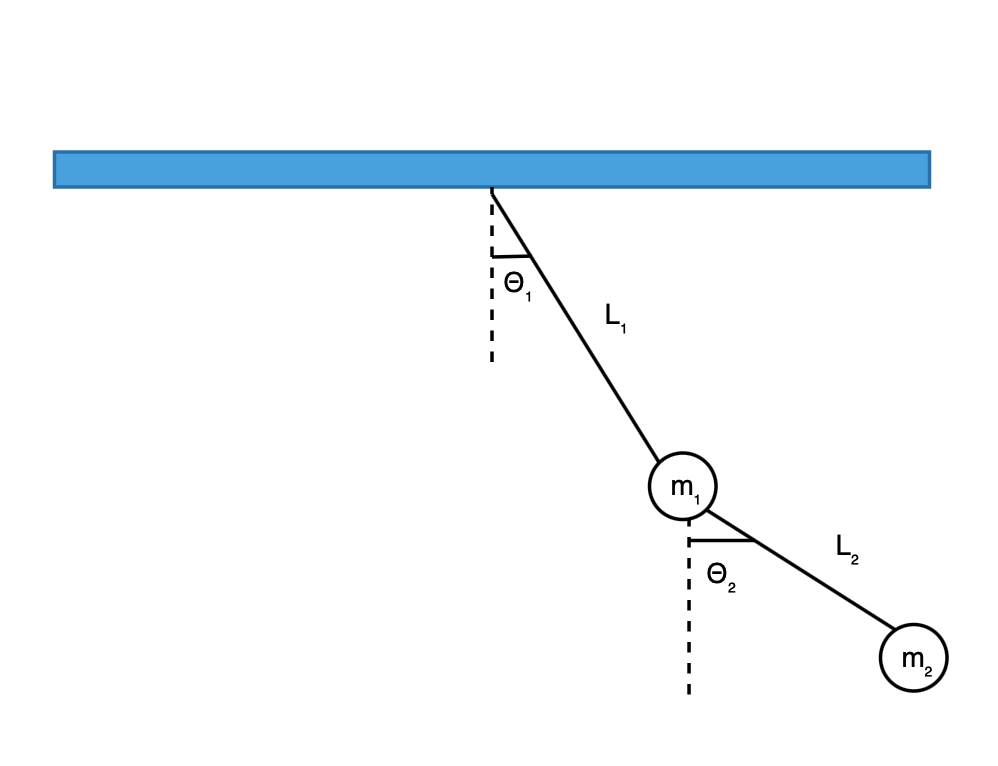
\includegraphics[width=0.6\textwidth]{../../../../datafiles/dblpend/dblpend.png}
\caption{The physical system}
\label{Figure:dblpend}
\end{center}
\end{figure}
\subsubsection{Goal Statements}
\label{Sec:GoalStmt}
Given the masses, length of the rods, initial angle of the masses and the gravitational constant, the goal statement is:

\begin{description}[font=\normalfont]
\item[motionMass:\phantomsection\label{motionMass}]{Calculate the motion of the masses.}
\end{description}
\subsection{Solution Characteristics Specification}
\label{Sec:SolCharSpec}
The instance models that govern DblPend are presented in the \hyperref[Sec:IMs]{Instance Model Section}. The information to understand the meaning of the instance models and their derivation is also presented, so that the instance models can be verified.

\subsubsection{Assumptions}
\label{Sec:Assumps}
This section simplifies the original problem and helps in developing the theoretical models by filling in the missing information for the physical system. The assumptions refine the scope by providing more detail.

\begin{description}[font=\normalfont]
\item[twoDMotion:\phantomsection\label{twoDMotion}]{The pendulum motion is two-dimensional (2D).}
\item[cartSys:\phantomsection\label{cartSys}]{A Cartesian coordinate system is used.}
\item[cartSysR:\phantomsection\label{cartSysR}]{The Cartesian coordinate system is right-handed where positive $x$-axis and $y$-axis point right up.}
\item[yAxisDir:\phantomsection\label{yAxisDir}]{The direction of the $y$-axis is directed opposite to gravity.}
\end{description}
\subsubsection{Theoretical Models}
\label{Sec:TMs}
This section focuses on the general equations and laws that DblPend is based on.

\medskip
\noindent
\begin{minipage}{\textwidth}
\begin{tabular}{>{\raggedright}p{0.13\textwidth}>{\raggedright\arraybackslash}p{0.82\textwidth}}
\toprule \textbf{Refname} & \textbf{TM:acceleration}
\phantomsection 
\label{TM:acceleration}
\\ \midrule
Label & Acceleration
        
\\ \midrule
Equation & \begin{displaymath}
           \resizeExpression{\symbf{a}\text{(}t\text{)}=\frac{\,d\symbf{v}\text{(}t\text{)}}{\,dt}}
           \end{displaymath}
\\ \midrule
Description & \begin{symbDescription}
              \item{$\symbf{a}\text{(}t\text{)}$ is the acceleration ($\frac{\text{m}}{\text{s}^{2}}$)}
              \item{$t$ is the time (${\text{s}}$)}
              \item{$\symbf{v}\text{(}t\text{)}$ is the velocity ($\frac{\text{m}}{\text{s}}$)}
              \end{symbDescription}
\\ \midrule
Source & \cite{accelerationWiki}
         
\\ \midrule
RefBy & 
\\ \bottomrule
\end{tabular}
\end{minipage}

\medskip
\noindent
\begin{minipage}{\textwidth}
\begin{tabular}{>{\raggedright}p{0.13\textwidth}>{\raggedright\arraybackslash}p{0.82\textwidth}}
\toprule \textbf{Refname} & \textbf{TM:velocity}
\phantomsection 
\label{TM:velocity}
\\ \midrule
Label & Velocity
        
\\ \midrule
Equation & \begin{displaymath}
           \resizeExpression{\symbf{v}\text{(}t\text{)}=\frac{\,d\symbf{p}\text{(}t\text{)}}{\,dt}}
           \end{displaymath}
\\ \midrule
Description & \begin{symbDescription}
              \item{$\symbf{v}\text{(}t\text{)}$ is the velocity ($\frac{\text{m}}{\text{s}}$)}
              \item{$t$ is the time (${\text{s}}$)}
              \item{$\symbf{p}\text{(}t\text{)}$ is the position (${\text{m}}$)}
              \end{symbDescription}
\\ \midrule
Source & \cite{velocityWiki}
         
\\ \midrule
RefBy & 
\\ \bottomrule
\end{tabular}
\end{minipage}

\medskip
\noindent
\begin{minipage}{\textwidth}
\begin{tabular}{>{\raggedright}p{0.13\textwidth}>{\raggedright\arraybackslash}p{0.82\textwidth}}
\toprule \textbf{Refname} & \textbf{TM:NewtonSecLawMot}
\phantomsection 
\label{TM:NewtonSecLawMot}
\\ \midrule
Label & Newton's second law of motion
        
\\ \midrule
Equation & \begin{displaymath}
           \resizeExpression{\symbf{F}=m\,\symbf{a}\text{(}t\text{)}}
           \end{displaymath}
\\ \midrule
Description & \begin{symbDescription}
              \item{$\symbf{F}$ is the force (${\text{N}}$)}
              \item{$m$ is the mass (${\text{kg}}$)}
              \item{$\symbf{a}\text{(}t\text{)}$ is the acceleration ($\frac{\text{m}}{\text{s}^{2}}$)}
              \end{symbDescription}
\\ \midrule
Notes & The net force $\symbf{F}$ on a body is proportional to the acceleration $\symbf{a}\text{(}t\text{)}$ of the body, where $m$ denotes the mass of the body as the constant of proportionality.
        
\\ \midrule
Source & --
         
\\ \midrule
RefBy & 
\\ \bottomrule
\end{tabular}
\end{minipage}

\subsubsection{General Definitions}
\label{Sec:GDs}
This section collects the laws and equations that will be used to build the instance models.

\medskip
\noindent
\begin{minipage}{\textwidth}
\begin{tabular}{>{\raggedright}p{0.13\textwidth}>{\raggedright\arraybackslash}p{0.82\textwidth}}
\toprule \textbf{Refname} & \textbf{GD:multivectorVelocity1}
\phantomsection 
\label{GD:multivectorVelocity1}
\\ \midrule
Label & Multivector velocity of the first object
        
\\ \midrule
Units & $\frac{\text{m}}{\text{s}}$
        
\\ \midrule
Equation & \begin{displaymath}
           \resizeExpression{{v_{1}}={w_{1}}\,{L_{1}} \begin{bmatrix}
                                                      \cos\left({θ_{1}}\right)\\
                                                      \sin\left({θ_{1}}\right)
                                                      \end{bmatrix}}
           \end{displaymath}
\\ \midrule
Description & \begin{symbDescription}
              \item{${v_{1}}$ is the velocity of the first object ($\frac{\text{m}}{\text{s}}$)}
              \item{${w_{1}}$ is the angular velocity of the first object ($\frac{\text{rad}}{\text{s}}$)}
              \item{${L_{1}}$ is the length of the first rod (${\text{m}}$)}
              \item{${θ_{1}}$ is the angle of the first rod (${\text{rad}}$)}
              \end{symbDescription}
\\ \midrule
Source & --
         
\\ \midrule
RefBy & 
\\ \bottomrule
\end{tabular}
\end{minipage}

\paragraph{Detailed derivation of velocity of the first object:}
\label{GD:multivectorVelocity1Deriv}
The multivector velocity in Clifford algebra represents both magnitude and direction as a unified geometric entity.

\begin{displaymath}
\resizeExpression{{v_{1}}={w_{1}}\,{L_{1}} \begin{bmatrix}
                                           \cos\left({θ_{1}}\right)\\
                                           \sin\left({θ_{1}}\right)
                                           \end{bmatrix}}
\end{displaymath}
Using the 2D Clifford space Cl(2,0), the velocity is expressed as a vector multivector with components in the e₁ and e₂ basis directions.

where the velocity multivector combines angular velocity and rod length in Clifford space

This approach provides a natural geometric representation that preserves rotational relationships.

Direction vector = cos(θ₁)e₁ + sin(θ₁)e₂ using basis vectors e₁, e₂

The angular velocity ω₁ and rod length L₁ combine with the direction vector to form the complete velocity multivector.

The geometric product preserves both magnitude and geometric orientation

Unlike traditional component-wise vector addition, this geometric product maintains the intrinsic geometric structure.

\medskip
\noindent
\begin{minipage}{\textwidth}
\begin{tabular}{>{\raggedright}p{0.13\textwidth}>{\raggedright\arraybackslash}p{0.82\textwidth}}
\toprule \textbf{Refname} & \textbf{GD:multivectorVelocity2}
\phantomsection 
\label{GD:multivectorVelocity2}
\\ \midrule
Label & Multivector velocity of the second object
        
\\ \midrule
Units & $\frac{\text{m}}{\text{s}}$
        
\\ \midrule
Equation & \begin{displaymath}
           \resizeExpression{{v_{2}}={w_{1}}\,{L_{1}} \begin{bmatrix}
                                                      \cos\left({θ_{1}}\right)\\
                                                      \sin\left({θ_{1}}\right)
                                                      \end{bmatrix}+{w_{2}}\,{L_{2}} \begin{bmatrix}
                                                                                     \cos\left({θ_{2}}\right)\\
                                                                                     \sin\left({θ_{2}}\right)
                                                                                     \end{bmatrix}}
           \end{displaymath}
\\ \midrule
Description & \begin{symbDescription}
              \item{${v_{2}}$ is the velocity of the second object ($\frac{\text{m}}{\text{s}}$)}
              \item{${w_{1}}$ is the angular velocity of the first object ($\frac{\text{rad}}{\text{s}}$)}
              \item{${L_{1}}$ is the length of the first rod (${\text{m}}$)}
              \item{${θ_{1}}$ is the angle of the first rod (${\text{rad}}$)}
              \item{${w_{2}}$ is the angular velocity of the second object ($\frac{\text{rad}}{\text{s}}$)}
              \item{${L_{2}}$ is the length of the second rod (${\text{m}}$)}
              \item{${θ_{2}}$ is the angle of the second rod (${\text{rad}}$)}
              \end{symbDescription}
\\ \midrule
Source & --
         
\\ \midrule
RefBy & 
\\ \bottomrule
\end{tabular}
\end{minipage}

\paragraph{Detailed derivation of velocity of the second object:}
\label{GD:multivectorVelocity2Deriv}
The multivector velocity for the second object combines the velocity from the first pendulum with its own rotational motion.

\begin{displaymath}
\resizeExpression{{v_{2}}={w_{1}}\,{L_{1}} \begin{bmatrix}
                                           \cos\left({θ_{1}}\right)\\
                                           \sin\left({θ_{1}}\right)
                                           \end{bmatrix}+{w_{2}}\,{L_{2}} \begin{bmatrix}
                                                                          \cos\left({θ_{2}}\right)\\
                                                                          \sin\left({θ_{2}}\right)
                                                                          \end{bmatrix}}
\end{displaymath}
In Clifford algebra, this vector addition preserves the geometric relationships between the two connected pendulums.

This represents the geometric sum of the first pendulum's velocity and the second pendulum's relative velocity

The total velocity is expressed as the sum of two vector multivectors in the same geometric space.

\medskip
\noindent
\begin{minipage}{\textwidth}
\begin{tabular}{>{\raggedright}p{0.13\textwidth}>{\raggedright\arraybackslash}p{0.82\textwidth}}
\toprule \textbf{Refname} & \textbf{GD:multivectorAcceleration1}
\phantomsection 
\label{GD:multivectorAcceleration1}
\\ \midrule
Label & Multivector acceleration of the first object
        
\\ \midrule
Units & $\frac{\text{m}}{\text{s}^{2}}$
        
\\ \midrule
Equation & \begin{displaymath}
           \resizeExpression{{a_{1}}={w_{1}}^{2}\,{L_{1}} \begin{bmatrix}
                                                          -\sin\left({θ_{1}}\right)\\
                                                          \cos\left({θ_{1}}\right)
                                                          \end{bmatrix}+{α_{1}}\,{L_{1}} \begin{bmatrix}
                                                                                         \cos\left({θ_{1}}\right)\\
                                                                                         \sin\left({θ_{1}}\right)
                                                                                         \end{bmatrix}}
           \end{displaymath}
\\ \midrule
Description & \begin{symbDescription}
              \item{${a_{1}}$ is the acceleration of the first object ($\frac{\text{m}}{\text{s}^{2}}$)}
              \item{${w_{1}}$ is the angular velocity of the first object ($\frac{\text{rad}}{\text{s}}$)}
              \item{${L_{1}}$ is the length of the first rod (${\text{m}}$)}
              \item{${θ_{1}}$ is the angle of the first rod (${\text{rad}}$)}
              \item{${α_{1}}$ is the angular acceleration of the first object ($\frac{\text{rad}}{\text{s}^{2}}$)}
              \end{symbDescription}
\\ \midrule
Source & --
         
\\ \midrule
RefBy & \hyperref[IM:calOfAngle2]{IM:calOfAngle2}
        
\\ \bottomrule
\end{tabular}
\end{minipage}

\paragraph{Detailed derivation of acceleration of the first object:}
\label{GD:multivectorAcceleration1Deriv}
The multivector acceleration in Clifford algebra combines centripetal and tangential acceleration components.

\begin{displaymath}
\resizeExpression{{a_{1}}={w_{1}}^{2}\,{L_{1}} \begin{bmatrix}
                                               -\sin\left({θ_{1}}\right)\\
                                               \cos\left({θ_{1}}\right)
                                               \end{bmatrix}+{α_{1}}\,{L_{1}} \begin{bmatrix}
                                                                              \cos\left({θ_{1}}\right)\\
                                                                              \sin\left({θ_{1}}\right)
                                                                              \end{bmatrix}}
\end{displaymath}
The centripetal acceleration points radially inward, while tangential acceleration is perpendicular to the rod.

where the acceleration combines centripetal and tangential components in Clifford space

Both components are naturally expressed as vector multivectors and added using Clifford geometric operations.

= centripetal\_multivector + tangential\_multivector

Centripetal component: -ω₁²L₁ × direction\_vector (radial inward)

Both terms maintain their geometric significance through the Clifford algebra representation

Tangential component: α₁L₁ × perpendicular\_direction\_vector (tangential)

The geometric sum preserves the underlying geometric relationships without component-wise decomposition.

\medskip
\noindent
\begin{minipage}{\textwidth}
\begin{tabular}{>{\raggedright}p{0.13\textwidth}>{\raggedright\arraybackslash}p{0.82\textwidth}}
\toprule \textbf{Refname} & \textbf{GD:multivectorAcceleration2}
\phantomsection 
\label{GD:multivectorAcceleration2}
\\ \midrule
Label & Multivector acceleration of the second object
        
\\ \midrule
Units & $\frac{\text{m}}{\text{s}^{2}}$
        
\\ \midrule
Equation & \begin{displaymath}
           \resizeExpression{{a_{2}}={w_{1}}^{2}\,{L_{1}} \begin{bmatrix}
                                                          -\sin\left({θ_{1}}\right)\\
                                                          \cos\left({θ_{1}}\right)
                                                          \end{bmatrix}+{α_{1}}\,{L_{1}} \begin{bmatrix}
                                                                                         \cos\left({θ_{1}}\right)\\
                                                                                         \sin\left({θ_{1}}\right)
                                                                                         \end{bmatrix}+{w_{2}}^{2}\,{L_{2}} \begin{bmatrix}
                                                                                                                            -\sin\left({θ_{2}}\right)\\
                                                                                                                            \cos\left({θ_{2}}\right)
                                                                                                                            \end{bmatrix}+{α_{2}}\,{L_{2}} \begin{bmatrix}
                                                                                                                                                           \cos\left({θ_{2}}\right)\\
                                                                                                                                                           \sin\left({θ_{2}}\right)
                                                                                                                                                           \end{bmatrix}}
           \end{displaymath}
\\ \midrule
Description & \begin{symbDescription}
              \item{${a_{2}}$ is the acceleration of the second object ($\frac{\text{m}}{\text{s}^{2}}$)}
              \item{${w_{1}}$ is the angular velocity of the first object ($\frac{\text{rad}}{\text{s}}$)}
              \item{${L_{1}}$ is the length of the first rod (${\text{m}}$)}
              \item{${θ_{1}}$ is the angle of the first rod (${\text{rad}}$)}
              \item{${α_{1}}$ is the angular acceleration of the first object ($\frac{\text{rad}}{\text{s}^{2}}$)}
              \item{${w_{2}}$ is the angular velocity of the second object ($\frac{\text{rad}}{\text{s}}$)}
              \item{${L_{2}}$ is the length of the second rod (${\text{m}}$)}
              \item{${θ_{2}}$ is the angle of the second rod (${\text{rad}}$)}
              \item{${α_{2}}$ is the angular acceleration of the second object ($\frac{\text{rad}}{\text{s}^{2}}$)}
              \end{symbDescription}
\\ \midrule
Source & --
         
\\ \midrule
RefBy & \hyperref[IM:calOfAngle2]{IM:calOfAngle2}
        
\\ \bottomrule
\end{tabular}
\end{minipage}

\paragraph{Detailed derivation of acceleration of the second object:}
\label{GD:multivectorAcceleration2Deriv}
The second object's acceleration is the geometric sum of the first object's acceleration and its own relative acceleration.

\begin{displaymath}
\resizeExpression{{a_{2}}={w_{1}}^{2}\,{L_{1}} \begin{bmatrix}
                                               -\sin\left({θ_{1}}\right)\\
                                               \cos\left({θ_{1}}\right)
                                               \end{bmatrix}+{α_{1}}\,{L_{1}} \begin{bmatrix}
                                                                              \cos\left({θ_{1}}\right)\\
                                                                              \sin\left({θ_{1}}\right)
                                                                              \end{bmatrix}+{w_{2}}^{2}\,{L_{2}} \begin{bmatrix}
                                                                                                                 -\sin\left({θ_{2}}\right)\\
                                                                                                                 \cos\left({θ_{2}}\right)
                                                                                                                 \end{bmatrix}+{α_{2}}\,{L_{2}} \begin{bmatrix}
                                                                                                                                                \cos\left({θ_{2}}\right)\\
                                                                                                                                                \sin\left({θ_{2}}\right)
                                                                                                                                                \end{bmatrix}}
\end{displaymath}
This captures the coupling between the two pendulums through their mechanical connection.

This represents the total acceleration as a vector sum in Clifford geometric space

The Clifford algebra representation preserves the geometric relationships in this coupled system.

\medskip
\noindent
\begin{minipage}{\textwidth}
\begin{tabular}{>{\raggedright}p{0.13\textwidth}>{\raggedright\arraybackslash}p{0.82\textwidth}}
\toprule \textbf{Refname} & \textbf{GD:multivectorForce1}
\phantomsection 
\label{GD:multivectorForce1}
\\ \midrule
Label & Multivector force on the first object
        
\\ \midrule
Units & ${\text{N}}$
        
\\ \midrule
Equation & \begin{displaymath}
           \resizeExpression{{f_{1}}={\symbf{T}_{1}} \begin{bmatrix}
                                                     -\sin\left({θ_{1}}\right)\\
                                                     \cos\left({θ_{1}}\right)
                                                     \end{bmatrix}+-\left({\symbf{T}_{2}} \begin{bmatrix}
                                                                                          -\sin\left({θ_{2}}\right)\\
                                                                                          \cos\left({θ_{2}}\right)
                                                                                          \end{bmatrix}\right)+\begin{bmatrix}
                                                                                                               0\\
                                                                                                               -{m_{1}}\,g
                                                                                                               \end{bmatrix}}
           \end{displaymath}
\\ \midrule
Description & \begin{symbDescription}
              \item{${f_{1}}$ is the force of the first object (${\text{N}}$)}
              \item{${\symbf{T}_{1}}$ is the tension of the first rod (${\text{N}}$)}
              \item{${θ_{1}}$ is the angle of the first rod (${\text{rad}}$)}
              \item{${\symbf{T}_{2}}$ is the tension of the second rod (${\text{N}}$)}
              \item{${θ_{2}}$ is the angle of the second rod (${\text{rad}}$)}
              \item{${m_{1}}$ is the mass of the first object (${\text{kg}}$)}
              \item{$g$ is the magnitude of gravitational acceleration ($\frac{\text{m}}{\text{s}^{2}}$)}
              \end{symbDescription}
\\ \midrule
Source & --
         
\\ \midrule
RefBy & \hyperref[IM:calOfAngle2]{IM:calOfAngle2}
        
\\ \bottomrule
\end{tabular}
\end{minipage}

\paragraph{Detailed derivation of force on the first object:}
\label{GD:multivectorForce1Deriv}
The multivector force in Clifford algebra combines inertial and gravitational forces as vector multivectors.

\begin{displaymath}
\resizeExpression{{f_{1}}={\symbf{T}_{1}} \begin{bmatrix}
                                          -\sin\left({θ_{1}}\right)\\
                                          \cos\left({θ_{1}}\right)
                                          \end{bmatrix}+-\left({\symbf{T}_{2}} \begin{bmatrix}
                                                                               -\sin\left({θ_{2}}\right)\\
                                                                               \cos\left({θ_{2}}\right)
                                                                               \end{bmatrix}\right)+\begin{bmatrix}
                                                                                                    0\\
                                                                                                    -{m_{1}}\,g
                                                                                                    \end{bmatrix}}
\end{displaymath}
The inertial force is proportional to the multivector acceleration, preserving Newton's second law in geometric form.

where force equals mass times acceleration plus gravitational force in vector form

Gravitational force acts vertically downward and is naturally represented as a vector multivector.

\medskip
\noindent
\begin{minipage}{\textwidth}
\begin{tabular}{>{\raggedright}p{0.13\textwidth}>{\raggedright\arraybackslash}p{0.82\textwidth}}
\toprule \textbf{Refname} & \textbf{GD:multivectorForce2}
\phantomsection 
\label{GD:multivectorForce2}
\\ \midrule
Label & Multivector force on the second object
        
\\ \midrule
Units & ${\text{N}}$
        
\\ \midrule
Equation & \begin{displaymath}
           \resizeExpression{{f_{2}}={\symbf{T}_{2}} \begin{bmatrix}
                                                     -\sin\left({θ_{2}}\right)\\
                                                     \cos\left({θ_{2}}\right)
                                                     \end{bmatrix}+\begin{bmatrix}
                                                                   0\\
                                                                   -{m_{2}}\,g
                                                                   \end{bmatrix}}
           \end{displaymath}
\\ \midrule
Description & \begin{symbDescription}
              \item{${f_{2}}$ is the force of the second object (${\text{N}}$)}
              \item{${\symbf{T}_{2}}$ is the tension of the second rod (${\text{N}}$)}
              \item{${θ_{2}}$ is the angle of the second rod (${\text{rad}}$)}
              \item{${m_{2}}$ is the mass of the second object (${\text{kg}}$)}
              \item{$g$ is the magnitude of gravitational acceleration ($\frac{\text{m}}{\text{s}^{2}}$)}
              \end{symbDescription}
\\ \midrule
Source & --
         
\\ \midrule
RefBy & \hyperref[IM:calOfAngle2]{IM:calOfAngle2}
        
\\ \bottomrule
\end{tabular}
\end{minipage}

\paragraph{Detailed derivation of force on the second object:}
\label{GD:multivectorForce2Deriv}
The force on the second object combines its inertial response with gravitational effects.

\begin{displaymath}
\resizeExpression{{f_{2}}={\symbf{T}_{2}} \begin{bmatrix}
                                          -\sin\left({θ_{2}}\right)\\
                                          \cos\left({θ_{2}}\right)
                                          \end{bmatrix}+\begin{bmatrix}
                                                        0\\
                                                        -{m_{2}}\,g
                                                        \end{bmatrix}}
\end{displaymath}
The Clifford algebra representation maintains the geometric consistency between force and acceleration.

This represents the total force as a vector sum in Clifford geometric space

This approach naturally handles the coupling forces between the connected pendulum objects.

= mass × acceleration\_multivector + gravitational\_force\_multivector

Key GA operations demonstrated: geometric product (combines magnitude and direction),

Demonstrating how Newton's second law extends naturally to geometric algebra

vector addition in Clifford space (preserves geometric relationships),

scalar multiplication with multivectors (maintains geometric structure).

\subsubsection{Data Definitions}
\label{Sec:DDs}
This section collects and defines all the data needed to build the instance models.

\medskip
\noindent
\begin{minipage}{\textwidth}
\begin{tabular}{>{\raggedright}p{0.13\textwidth}>{\raggedright\arraybackslash}p{0.82\textwidth}}
\toprule \textbf{Refname} & \textbf{DD:velocityGDD}
\phantomsection 
\label{DD:velocityGDD}
\\ \midrule
Label & Velocity
        
\\ \midrule
Symbol & $\symbf{v}\text{(}t\text{)}$
         
\\ \midrule
Units & $\frac{\text{m}}{\text{s}}$
        
\\ \midrule
Equation & \begin{displaymath}
           \resizeExpression{\symbf{v}\text{(}t\text{)}=\frac{\,d\symbf{p}\text{(}t\text{)}}{\,dt}}
           \end{displaymath}
\\ \midrule
Description & \begin{symbDescription}
              \item{$\symbf{v}\text{(}t\text{)}$ is the velocity ($\frac{\text{m}}{\text{s}}$)}
              \item{$t$ is the time (${\text{s}}$)}
              \item{$\symbf{p}\text{(}t\text{)}$ is the position (${\text{m}}$)}
              \end{symbDescription}
\\ \midrule
Source & --
         
\\ \midrule
RefBy & 
\\ \bottomrule
\end{tabular}
\end{minipage}

\medskip
\noindent
\begin{minipage}{\textwidth}
\begin{tabular}{>{\raggedright}p{0.13\textwidth}>{\raggedright\arraybackslash}p{0.82\textwidth}}
\toprule \textbf{Refname} & \textbf{DD:positionXDD1}
\phantomsection 
\label{DD:positionXDD1}
\\ \midrule
Label & Horizontal position of the first object
        
\\ \midrule
Symbol & ${p_{\text{x}1}}$
         
\\ \midrule
Units & ${\text{m}}$
        
\\ \midrule
Equation & \begin{displaymath}
           \resizeExpression{{p_{\text{x}1}}={L_{1}}\,\sin\left({θ_{1}}\right)}
           \end{displaymath}
\\ \midrule
Description & \begin{symbDescription}
              \item{${p_{\text{x}1}}$ is the horizontal position of the first object (${\text{m}}$)}
              \item{${L_{1}}$ is the length of the first rod (${\text{m}}$)}
              \item{${θ_{1}}$ is the angle of the first rod (${\text{rad}}$)}
              \end{symbDescription}
\\ \midrule
Notes & ${p_{\text{x}1}}$ is the horizontal position
        
        ${p_{\text{x}1}}$ is shown in \hyperref[Figure:dblpend]{Fig:dblpend}.
        
\\ \midrule
Source & --
         
\\ \midrule
RefBy & 
\\ \bottomrule
\end{tabular}
\end{minipage}

\medskip
\noindent
\begin{minipage}{\textwidth}
\begin{tabular}{>{\raggedright}p{0.13\textwidth}>{\raggedright\arraybackslash}p{0.82\textwidth}}
\toprule \textbf{Refname} & \textbf{DD:positionYDD1}
\phantomsection 
\label{DD:positionYDD1}
\\ \midrule
Label & Vertical position of the first object
        
\\ \midrule
Symbol & ${p_{\text{y}1}}$
         
\\ \midrule
Units & ${\text{m}}$
        
\\ \midrule
Equation & \begin{displaymath}
           \resizeExpression{{p_{\text{y}1}}=-{L_{1}}\,\cos\left({θ_{1}}\right)}
           \end{displaymath}
\\ \midrule
Description & \begin{symbDescription}
              \item{${p_{\text{y}1}}$ is the vertical position of the first object (${\text{m}}$)}
              \item{${L_{1}}$ is the length of the first rod (${\text{m}}$)}
              \item{${θ_{1}}$ is the angle of the first rod (${\text{rad}}$)}
              \end{symbDescription}
\\ \midrule
Notes & ${p_{\text{y}1}}$ is the vertical position
        
        ${p_{\text{y}1}}$ is shown in \hyperref[Figure:dblpend]{Fig:dblpend}.
        
\\ \midrule
Source & --
         
\\ \midrule
RefBy & 
\\ \bottomrule
\end{tabular}
\end{minipage}

\medskip
\noindent
\begin{minipage}{\textwidth}
\begin{tabular}{>{\raggedright}p{0.13\textwidth}>{\raggedright\arraybackslash}p{0.82\textwidth}}
\toprule \textbf{Refname} & \textbf{DD:positionXDD2}
\phantomsection 
\label{DD:positionXDD2}
\\ \midrule
Label & Horizontal position of the second object
        
\\ \midrule
Symbol & ${p_{\text{x}2}}$
         
\\ \midrule
Units & ${\text{m}}$
        
\\ \midrule
Equation & \begin{displaymath}
           \resizeExpression{{p_{\text{x}2}}={p_{\text{x}1}}+{L_{2}}\,\sin\left({θ_{2}}\right)}
           \end{displaymath}
\\ \midrule
Description & \begin{symbDescription}
              \item{${p_{\text{x}2}}$ is the horizontal position of the second object (${\text{m}}$)}
              \item{${p_{\text{x}1}}$ is the horizontal position of the first object (${\text{m}}$)}
              \item{${L_{2}}$ is the length of the second rod (${\text{m}}$)}
              \item{${θ_{2}}$ is the angle of the second rod (${\text{rad}}$)}
              \end{symbDescription}
\\ \midrule
Notes & ${p_{\text{x}2}}$ is the horizontal position
        
        ${p_{\text{x}2}}$ is shown in \hyperref[Figure:dblpend]{Fig:dblpend}.
        
\\ \midrule
Source & --
         
\\ \midrule
RefBy & 
\\ \bottomrule
\end{tabular}
\end{minipage}

\medskip
\noindent
\begin{minipage}{\textwidth}
\begin{tabular}{>{\raggedright}p{0.13\textwidth}>{\raggedright\arraybackslash}p{0.82\textwidth}}
\toprule \textbf{Refname} & \textbf{DD:positionYDD2}
\phantomsection 
\label{DD:positionYDD2}
\\ \midrule
Label & Vertical position of the second object
        
\\ \midrule
Symbol & ${p_{\text{y}2}}$
         
\\ \midrule
Units & ${\text{m}}$
        
\\ \midrule
Equation & \begin{displaymath}
           \resizeExpression{{p_{\text{y}2}}={p_{\text{y}1}}-{L_{2}}\,\cos\left({θ_{2}}\right)}
           \end{displaymath}
\\ \midrule
Description & \begin{symbDescription}
              \item{${p_{\text{y}2}}$ is the vertical position of the second object (${\text{m}}$)}
              \item{${p_{\text{y}1}}$ is the vertical position of the first object (${\text{m}}$)}
              \item{${L_{2}}$ is the length of the second rod (${\text{m}}$)}
              \item{${θ_{2}}$ is the angle of the second rod (${\text{rad}}$)}
              \end{symbDescription}
\\ \midrule
Notes & ${p_{\text{y}2}}$ is the vertical position
        
        ${p_{\text{y}2}}$ is shown in \hyperref[Figure:dblpend]{Fig:dblpend}.
        
\\ \midrule
Source & --
         
\\ \midrule
RefBy & 
\\ \bottomrule
\end{tabular}
\end{minipage}

\medskip
\noindent
\begin{minipage}{\textwidth}
\begin{tabular}{>{\raggedright}p{0.13\textwidth}>{\raggedright\arraybackslash}p{0.82\textwidth}}
\toprule \textbf{Refname} & \textbf{DD:accelerationGDD}
\phantomsection 
\label{DD:accelerationGDD}
\\ \midrule
Label & Acceleration
        
\\ \midrule
Symbol & $\symbf{a}\text{(}t\text{)}$
         
\\ \midrule
Units & $\frac{\text{m}}{\text{s}^{2}}$
        
\\ \midrule
Equation & \begin{displaymath}
           \resizeExpression{\symbf{a}\text{(}t\text{)}=\frac{\,d\symbf{v}\text{(}t\text{)}}{\,dt}}
           \end{displaymath}
\\ \midrule
Description & \begin{symbDescription}
              \item{$\symbf{a}\text{(}t\text{)}$ is the acceleration ($\frac{\text{m}}{\text{s}^{2}}$)}
              \item{$t$ is the time (${\text{s}}$)}
              \item{$\symbf{v}\text{(}t\text{)}$ is the velocity ($\frac{\text{m}}{\text{s}}$)}
              \end{symbDescription}
\\ \midrule
Source & --
         
\\ \midrule
RefBy & 
\\ \bottomrule
\end{tabular}
\end{minipage}

\medskip
\noindent
\begin{minipage}{\textwidth}
\begin{tabular}{>{\raggedright}p{0.13\textwidth}>{\raggedright\arraybackslash}p{0.82\textwidth}}
\toprule \textbf{Refname} & \textbf{DD:forceGDD}
\phantomsection 
\label{DD:forceGDD}
\\ \midrule
Label & Force
        
\\ \midrule
Symbol & $\symbf{F}$
         
\\ \midrule
Units & ${\text{N}}$
        
\\ \midrule
Equation & \begin{displaymath}
           \resizeExpression{\symbf{F}=m \symbf{a}\text{(}t\text{)}}
           \end{displaymath}
\\ \midrule
Description & \begin{symbDescription}
              \item{$\symbf{F}$ is the force (${\text{N}}$)}
              \item{$m$ is the mass (${\text{kg}}$)}
              \item{$\symbf{a}\text{(}t\text{)}$ is the acceleration ($\frac{\text{m}}{\text{s}^{2}}$)}
              \end{symbDescription}
\\ \midrule
Source & --
         
\\ \midrule
RefBy & 
\\ \bottomrule
\end{tabular}
\end{minipage}

\subsubsection{Instance Models}
\label{Sec:IMs}
This section transforms the problem defined in the \hyperref[Sec:ProbDesc]{problem description} into one which is expressed in mathematical terms. It uses concrete symbols defined in the \hyperref[Sec:DDs]{data definitions} to replace the abstract symbols in the models identified in \hyperref[Sec:TMs]{theoretical models} and \hyperref[Sec:GDs]{general definitions}.

\medskip
\noindent
\begin{minipage}{\textwidth}
\begin{tabular}{>{\raggedright}p{0.13\textwidth}>{\raggedright\arraybackslash}p{0.82\textwidth}}
\toprule \textbf{Refname} & \textbf{IM:calOfAngle1}
\phantomsection 
\label{IM:calOfAngle1}
\\ \midrule
Label & Calculation of angle of first rod
        
\\ \midrule
Input & ${L_{1}}$, ${L_{2}}$, ${m_{1}}$, ${m_{2}}$, ${θ_{1}}$, ${θ_{2}}$
        
\\ \midrule
Output & ${θ_{1}}$
         
\\ \midrule
Input Constraints & \begin{displaymath}
                    \resizeExpression{{L_{1}}\gt{}0}
                    \end{displaymath}
                    \begin{displaymath}
                    \resizeExpression{{L_{2}}\gt{}0}
                    \end{displaymath}
                    \begin{displaymath}
                    \resizeExpression{{m_{1}}\gt{}0}
                    \end{displaymath}
                    \begin{displaymath}
                    \resizeExpression{{m_{2}}\gt{}0}
                    \end{displaymath}
\\ \midrule
Output Constraints & 
\\ \midrule
Equation & \begin{displaymath}
           \resizeExpression{{α_{1}}\left({θ_{1}},{θ_{2}},{w_{1}},{w_{2}}\right)=\frac{-g\,\left(2\,{m_{1}}+{m_{2}}\right)\,\sin\left({θ_{1}}\right)-{m_{2}}\,g\,\sin\left({θ_{1}}-2\,{θ_{2}}\right)-2\,\sin\left({θ_{1}}-{θ_{2}}\right)\,{m_{2}}\,\left({w_{2}}^{2}\,{L_{2}}+{w_{1}}^{2}\,{L_{1}}\,\cos\left({θ_{1}}-{θ_{2}}\right)\right)}{{L_{1}}\,\left(2\,{m_{1}}+{m_{2}}-{m_{2}}\,\cos\left(2\,{θ_{1}}-2\,{θ_{2}}\right)\right)}}
           \end{displaymath}
\\ \midrule
Description & \begin{symbDescription}
              \item{${α_{1}}$ is the angular acceleration of the first object ($\frac{\text{rad}}{\text{s}^{2}}$)}
              \item{${θ_{1}}$ is the angle of the first rod (${\text{rad}}$)}
              \item{${θ_{2}}$ is the angle of the second rod (${\text{rad}}$)}
              \item{${w_{1}}$ is the angular velocity of the first object ($\frac{\text{rad}}{\text{s}}$)}
              \item{${w_{2}}$ is the angular velocity of the second object ($\frac{\text{rad}}{\text{s}}$)}
              \item{$g$ is the magnitude of gravitational acceleration ($\frac{\text{m}}{\text{s}^{2}}$)}
              \item{${m_{1}}$ is the mass of the first object (${\text{kg}}$)}
              \item{${m_{2}}$ is the mass of the second object (${\text{kg}}$)}
              \item{${L_{2}}$ is the length of the second rod (${\text{m}}$)}
              \item{${L_{1}}$ is the length of the first rod (${\text{m}}$)}
              \end{symbDescription}
\\ \midrule
Notes & ${θ_{1}}$ is calculated by solving the ODE here together with the initial conditions and \hyperref[IM:calOfAngle2]{IM:calOfAngle2}.
        
\\ \midrule
Source & --
         
\\ \midrule
RefBy & \hyperref[IM:calOfAngle2]{IM:calOfAngle2}, \hyperref[outputValues]{FR:Output-Values}, and \hyperref[calcAng]{FR:Calculate-Angle-Of-Rod}
        
\\ \bottomrule
\end{tabular}
\end{minipage}

\medskip
\noindent
\begin{minipage}{\textwidth}
\begin{tabular}{>{\raggedright}p{0.13\textwidth}>{\raggedright\arraybackslash}p{0.82\textwidth}}
\toprule \textbf{Refname} & \textbf{IM:calOfAngle2}
\phantomsection 
\label{IM:calOfAngle2}
\\ \midrule
Label & Calculation of angle of second rod
        
\\ \midrule
Input & ${L_{1}}$, ${L_{2}}$, ${m_{1}}$, ${m_{2}}$, ${θ_{1}}$, ${θ_{2}}$
        
\\ \midrule
Output & ${θ_{2}}$
         
\\ \midrule
Input Constraints & \begin{displaymath}
                    \resizeExpression{{L_{1}}\gt{}0}
                    \end{displaymath}
                    \begin{displaymath}
                    \resizeExpression{{L_{2}}\gt{}0}
                    \end{displaymath}
                    \begin{displaymath}
                    \resizeExpression{{m_{1}}\gt{}0}
                    \end{displaymath}
                    \begin{displaymath}
                    \resizeExpression{{m_{2}}\gt{}0}
                    \end{displaymath}
\\ \midrule
Output Constraints & 
\\ \midrule
Equation & \begin{displaymath}
           \resizeExpression{{α_{2}}\left({θ_{1}},{θ_{2}},{w_{1}},{w_{2}}\right)=\frac{2\,\sin\left({θ_{1}}-{θ_{2}}\right)\,\left({w_{1}}^{2}\,{L_{1}}\,\left({m_{1}}+{m_{2}}\right)+g\,\left({m_{1}}+{m_{2}}\right)\,\cos\left({θ_{1}}\right)+{w_{2}}^{2}\,{L_{2}}\,{m_{2}}\,\cos\left({θ_{1}}-{θ_{2}}\right)\right)}{{L_{2}}\,\left(2\,{m_{1}}+{m_{2}}-{m_{2}}\,\cos\left(2\,{θ_{1}}-2\,{θ_{2}}\right)\right)}}
           \end{displaymath}
\\ \midrule
Description & \begin{symbDescription}
              \item{${α_{2}}$ is the angular acceleration of the second object ($\frac{\text{rad}}{\text{s}^{2}}$)}
              \item{${θ_{1}}$ is the angle of the first rod (${\text{rad}}$)}
              \item{${θ_{2}}$ is the angle of the second rod (${\text{rad}}$)}
              \item{${w_{1}}$ is the angular velocity of the first object ($\frac{\text{rad}}{\text{s}}$)}
              \item{${w_{2}}$ is the angular velocity of the second object ($\frac{\text{rad}}{\text{s}}$)}
              \item{${L_{1}}$ is the length of the first rod (${\text{m}}$)}
              \item{${m_{1}}$ is the mass of the first object (${\text{kg}}$)}
              \item{${m_{2}}$ is the mass of the second object (${\text{kg}}$)}
              \item{$g$ is the magnitude of gravitational acceleration ($\frac{\text{m}}{\text{s}^{2}}$)}
              \item{${L_{2}}$ is the length of the second rod (${\text{m}}$)}
              \end{symbDescription}
\\ \midrule
Notes & ${θ_{2}}$ is calculated by solving the ODE here together with the initial conditions and \hyperref[IM:calOfAngle1]{IM:calOfAngle1}.
        
\\ \midrule
Source & --
         
\\ \midrule
RefBy & \hyperref[IM:calOfAngle2]{IM:calOfAngle2}, \hyperref[IM:calOfAngle1]{IM:calOfAngle1}, \hyperref[outputValues]{FR:Output-Values}, and \hyperref[calcAng]{FR:Calculate-Angle-Of-Rod}
        
\\ \bottomrule
\end{tabular}
\end{minipage}

\paragraph{Detailed derivation of angle of the second rod:}
\label{IM:calOfAngle2Deriv}
By solving multivector force equations \hyperref[GD:multivectorForce1]{GD:multivectorForce1} and \hyperref[GD:multivectorForce2]{GD:multivectorForce2} for ${f_{1}}$ and ${f_{2}}$ and then substituting into the Clifford algebra force equations , we can get equations 1 and 2:

\begin{displaymath}
\resizeExpression{{m_{1}}\,{a_{1}}=-{\symbf{T}_{1}}\,\sin\left({θ_{1}}\right)-{m_{2}}\,{a_{2}}}
\end{displaymath}

\begin{displaymath}
\resizeExpression{{m_{1}}\,{a_{1}}={\symbf{T}_{1}}\,\cos\left({θ_{1}}\right)-{m_{2}}\,{a_{2}}-{m_{2}}\,g-{m_{1}}\,g}
\end{displaymath}
Multiply the equation 1 by $\cos\left({θ_{1}}\right)$ and the equation 2 by $\sin\left({θ_{1}}\right)$ and rearrange to get:

\begin{displaymath}
\resizeExpression{{\symbf{T}_{1}}\,\sin\left({θ_{1}}\right)\,\cos\left({θ_{1}}\right)=-\cos\left({θ_{1}}\right)\,\left({m_{1}}\,{a_{1}}+{m_{2}}\,{a_{2}}\right)}
\end{displaymath}

\begin{displaymath}
\resizeExpression{{\symbf{T}_{1}}\,\sin\left({θ_{1}}\right)\,\cos\left({θ_{1}}\right)=\sin\left({θ_{1}}\right)\,\left({m_{1}}\,{a_{1}}+{m_{2}}\,{a_{2}}+{m_{2}}\,g+{m_{1}}\,g\right)}
\end{displaymath}
This leads to the equation 3

\begin{displaymath}
\resizeExpression{\sin\left({θ_{1}}\right)\,\left({m_{1}}\,{a_{1}}+{m_{2}}\,{a_{2}}+{m_{2}}\,g+{m_{1}}\,g\right)=-\cos\left({θ_{1}}\right)\,\left({m_{1}}\,{a_{1}}+{m_{2}}\,{a_{2}}\right)}
\end{displaymath}
Next, multiply multivector force equation \hyperref[GD:multivectorForce2]{GD:multivectorForce2} by $\cos\left({θ_{2}}\right)$ and the Clifford force equation by $\sin\left({θ_{2}}\right)$ and rearrange to get:

\begin{displaymath}
\resizeExpression{{\symbf{T}_{2}}\,\sin\left({θ_{2}}\right)\,\cos\left({θ_{2}}\right)=-\cos\left({θ_{2}}\right)\,{m_{2}}\,{a_{2}}}
\end{displaymath}

\begin{displaymath}
\resizeExpression{{\symbf{T}_{2}}\,\sin\left({θ_{2}}\right)\,\cos\left({θ_{2}}\right)=\sin\left({θ_{2}}\right)\,\left({m_{2}}\,{a_{2}}+{m_{2}}\,g\right)}
\end{displaymath}
which leads to equation 4

\begin{displaymath}
\resizeExpression{\sin\left({θ_{2}}\right)\,\left({m_{2}}\,{a_{2}}+{m_{2}}\,g\right)=-\cos\left({θ_{2}}\right)\,{m_{2}}\,{a_{2}}}
\end{displaymath}
By giving multivector acceleration equations \hyperref[GD:multivectorAcceleration1]{GD:multivectorAcceleration1} and \hyperref[GD:multivectorAcceleration2]{GD:multivectorAcceleration2} and plus Clifford algebra equations plus additional two equations, 3 and 4, we can get \hyperref[IM:calOfAngle1]{IM:calOfAngle1} and \hyperref[IM:calOfAngle2]{IM:calOfAngle2} via a computer algebra program:

\subsubsection{Data Constraints}
\label{Sec:DataConstraints}
The \hyperref[Table:InDataConstraints]{Data Constraints Table} shows the data constraints on the input variables. The column for physical constraints gives the physical limitations on the range of values that can be taken by the variable. The uncertainty column provides an estimate of the confidence with which the physical quantities can be measured. This information would be part of the input if one were performing an uncertainty quantification exercise. The constraints are conservative to give the user of the model the flexibility to experiment with unusual situations. The column of typical values is intended to provide a feel for a common scenario.

\begin{longtblr}
[caption={Input Data Constraints}]
{colspec={l l l l}, rowhead=1, hline{1,Z}=\heavyrulewidth, hline{2}=\lightrulewidth}
\textbf{Var} & \textbf{Physical Constraints} & \textbf{Typical Value} & \textbf{Uncert.}
\\
${L_{1}}$ & ${L_{1}}\gt{}0$ & $1.0$ ${\text{m}}$ & 10$\%$
\\
${L_{2}}$ & ${L_{2}}\gt{}0$ & $1.0$ ${\text{m}}$ & 10$\%$
\\
${m_{1}}$ & ${m_{1}}\gt{}0$ & $0.5$ ${\text{kg}}$ & 10$\%$
\\
${m_{2}}$ & ${m_{2}}\gt{}0$ & $0.5$ ${\text{kg}}$ & 10$\%$
\label{Table:InDataConstraints}
\end{longtblr}
\subsubsection{Properties of a Correct Solution}
\label{Sec:CorSolProps}
The \hyperref[Table:OutDataConstraints]{Data Constraints Table} shows the data constraints on the output variables. The column for physical constraints gives the physical limitations on the range of values that can be taken by the variable.

\begin{longtblr}
[caption={Output Data Constraints}]
{colspec={l l}, rowhead=1, hline{1,Z}=\heavyrulewidth, hline{2}=\lightrulewidth}
\textbf{Var} & \textbf{Physical Constraints}
\\
${θ_{1}}$ & ${θ_{1}}\gt{}0$
\\
${θ_{2}}$ & ${θ_{2}}\gt{}0$
\label{Table:OutDataConstraints}
\end{longtblr}
\section{Requirements}
\label{Sec:Requirements}
This section provides the functional requirements, the tasks and behaviours that the software is expected to complete, and the non-functional requirements, the qualities that the software is expected to exhibit.

\subsection{Functional Requirements}
\label{Sec:FRs}
This section provides the functional requirements, the tasks and behaviours that the software is expected to complete.

\begin{description}[font=\normalfont]
\item[Input-Values:\phantomsection\label{inputValues}]{Input the values from \hyperref[Table:ReqInputs]{Tab:ReqInputs}.}
\item[Verify-Input-Values:\phantomsection\label{verifyInptVals}]{Check the entered input values to ensure that they do not exceed the \hyperref[Sec:DataConstraints]{data constraints}. If any of the input values are out of bounds, an error message is displayed and the calculations stop.}
\item[Calculate-Angle-Of-Rod:\phantomsection\label{calcAng}]{Calculate the following values: ${θ_{1}}$ and ${θ_{2}}$ (from \hyperref[IM:calOfAngle1]{IM:calOfAngle1} and \hyperref[IM:calOfAngle2]{IM:calOfAngle2}).}
\item[Output-Values:\phantomsection\label{outputValues}]{Output ${θ_{1}}$ and ${θ_{2}}$ (from \hyperref[IM:calOfAngle1]{IM:calOfAngle1} and \hyperref[IM:calOfAngle2]{IM:calOfAngle2}).}
\end{description}
\begin{longtblr}
[caption={Required Inputs}]
{colspec={l l l}, rowhead=1, hline{1,Z}=\heavyrulewidth, hline{2}=\lightrulewidth}
\textbf{Symbol} & \textbf{Description} & \textbf{Units}
\\
${L_{1}}$ & Length of the first rod & ${\text{m}}$
\\
${L_{2}}$ & Length of the second rod & ${\text{m}}$
\\
${m_{1}}$ & Mass of the first object & ${\text{kg}}$
\\
${m_{2}}$ & Mass of the second object & ${\text{kg}}$
\\
${θ_{1}}$ & Angle of the first rod & ${\text{rad}}$
\\
${θ_{2}}$ & Angle of the second rod & ${\text{rad}}$
\label{Table:ReqInputs}
\end{longtblr}
\subsection{Non-Functional Requirements}
\label{Sec:NFRs}
This section provides the non-functional requirements, the qualities that the software is expected to exhibit.

\begin{description}[font=\normalfont]
\item[Correctness:\phantomsection\label{correct}]{The outputs of the code have the \hyperref[Sec:CorSolProps]{properties of a correct solution}.}
\item[Portability:\phantomsection\label{portable}]{The code shall be portable to multiple environments, particularly Windows, Mac OSX, and Linux.}
\end{description}
\section{Traceability Matrices and Graphs}
\label{Sec:TraceMatrices}
The purpose of the traceability matrices is to provide easy references on what has to be additionally modified if a certain component is changed. Every time a component is changed, the items in the column of that component that are marked with an ``X'' should be modified as well. \hyperref[Table:TraceMatAvsA]{Tab:TraceMatAvsA} shows the dependencies of the assumptions on each other. \hyperref[Table:TraceMatAvsAll]{Tab:TraceMatAvsAll} shows the dependencies of the data definitions, theoretical models, general definitions, instance models, requirements, likely changes, and unlikely changes on the assumptions. \hyperref[Table:TraceMatRefvsRef]{Tab:TraceMatRefvsRef} shows the dependencies of the data definitions, theoretical models, general definitions, and instance models on each other. \hyperref[Table:TraceMatAllvsR]{Tab:TraceMatAllvsR} shows the dependencies of the requirements and goal statements on the data definitions, theoretical models, general definitions, and instance models.

\begin{longtblr}
[caption={Traceability Matrix Showing the Connections Between Assumptions and Other Assumptions}]
{colspec={l l l l l}, rowhead=1, hline{1,Z}=\heavyrulewidth, hline{2}=\lightrulewidth}
\textbf{} & \textbf{\hyperref[twoDMotion]{A:twoDMotion}} & \textbf{\hyperref[cartSys]{A:cartSys}} & \textbf{\hyperref[cartSysR]{A:cartSysR}} & \textbf{\hyperref[yAxisDir]{A:yAxisDir}}
\\
\hyperref[twoDMotion]{A:twoDMotion} &  &  &  & 
\\
\hyperref[cartSys]{A:cartSys} &  &  &  & 
\\
\hyperref[cartSysR]{A:cartSysR} &  &  &  & 
\\
\hyperref[yAxisDir]{A:yAxisDir} &  &  &  & 
\label{Table:TraceMatAvsA}
\end{longtblr}
\begin{longtblr}
[caption={Traceability Matrix Showing the Connections Between Assumptions and Other Items}]
{colspec={l l l l l}, rowhead=1, hline{1,Z}=\heavyrulewidth, hline{2}=\lightrulewidth}
\textbf{} & \textbf{\hyperref[twoDMotion]{A:twoDMotion}} & \textbf{\hyperref[cartSys]{A:cartSys}} & \textbf{\hyperref[cartSysR]{A:cartSysR}} & \textbf{\hyperref[yAxisDir]{A:yAxisDir}}
\\
\hyperref[DD:velocityGDD]{DD:velocityGDD} &  &  &  & 
\\
\hyperref[DD:positionXDD1]{DD:positionXDD1} &  &  &  & 
\\
\hyperref[DD:positionYDD1]{DD:positionYDD1} &  &  &  & 
\\
\hyperref[DD:positionXDD2]{DD:positionXDD2} &  &  &  & 
\\
\hyperref[DD:positionYDD2]{DD:positionYDD2} &  &  &  & 
\\
\hyperref[DD:accelerationGDD]{DD:accelerationGDD} &  &  &  & 
\\
\hyperref[DD:forceGDD]{DD:forceGDD} &  &  &  & 
\\
\hyperref[TM:acceleration]{TM:acceleration} &  &  &  & 
\\
\hyperref[TM:velocity]{TM:velocity} &  &  &  & 
\\
\hyperref[TM:NewtonSecLawMot]{TM:NewtonSecLawMot} &  &  &  & 
\\
\hyperref[GD:multivectorVelocity1]{GD:multivectorVelocity1} &  &  &  & 
\\
\hyperref[GD:multivectorVelocity2]{GD:multivectorVelocity2} &  &  &  & 
\\
\hyperref[GD:multivectorAcceleration1]{GD:multivectorAcceleration1} &  &  &  & 
\\
\hyperref[GD:multivectorAcceleration2]{GD:multivectorAcceleration2} &  &  &  & 
\\
\hyperref[GD:multivectorForce1]{GD:multivectorForce1} &  &  &  & 
\\
\hyperref[GD:multivectorForce2]{GD:multivectorForce2} &  &  &  & 
\\
\hyperref[IM:calOfAngle1]{IM:calOfAngle1} &  &  &  & 
\\
\hyperref[IM:calOfAngle2]{IM:calOfAngle2} &  &  &  & 
\\
\hyperref[correct]{NFR:Correctness} &  &  &  & 
\\
\hyperref[portable]{NFR:Portability} &  &  &  & 
\\
\hyperref[inputValues]{FR:Input-Values} &  &  &  & 
\\
\hyperref[verifyInptVals]{FR:Verify-Input-Values} &  &  &  & 
\\
\hyperref[calcAng]{FR:Calculate-Angle-Of-Rod} &  &  &  & 
\\
\hyperref[outputValues]{FR:Output-Values} &  &  &  & 
\label{Table:TraceMatAvsAll}
\end{longtblr}
\begin{longtblr}
[caption={Traceability Matrix Showing the Connections Between Items and Other Sections}]
{colspec={l l l l l l l l l l l l l l l l l l l}, rowhead=1, hline{1,Z}=\heavyrulewidth, hline{2}=\lightrulewidth}
\textbf{} & \textbf{\hyperref[DD:velocityGDD]{DD:velocityGDD}} & \textbf{\hyperref[DD:positionXDD1]{DD:positionXDD1}} & \textbf{\hyperref[DD:positionYDD1]{DD:positionYDD1}} & \textbf{\hyperref[DD:positionXDD2]{DD:positionXDD2}} & \textbf{\hyperref[DD:positionYDD2]{DD:positionYDD2}} & \textbf{\hyperref[DD:accelerationGDD]{DD:accelerationGDD}} & \textbf{\hyperref[DD:forceGDD]{DD:forceGDD}} & \textbf{\hyperref[TM:acceleration]{TM:acceleration}} & \textbf{\hyperref[TM:velocity]{TM:velocity}} & \textbf{\hyperref[TM:NewtonSecLawMot]{TM:NewtonSecLawMot}} & \textbf{\hyperref[GD:multivectorVelocity1]{GD:multivectorVelocity1}} & \textbf{\hyperref[GD:multivectorVelocity2]{GD:multivectorVelocity2}} & \textbf{\hyperref[GD:multivectorAcceleration1]{GD:multivectorAcceleration1}} & \textbf{\hyperref[GD:multivectorAcceleration2]{GD:multivectorAcceleration2}} & \textbf{\hyperref[GD:multivectorForce1]{GD:multivectorForce1}} & \textbf{\hyperref[GD:multivectorForce2]{GD:multivectorForce2}} & \textbf{\hyperref[IM:calOfAngle1]{IM:calOfAngle1}} & \textbf{\hyperref[IM:calOfAngle2]{IM:calOfAngle2}}
\\
\hyperref[DD:velocityGDD]{DD:velocityGDD} &  &  &  &  &  &  &  &  &  &  &  &  &  &  &  &  &  & 
\\
\hyperref[DD:positionXDD1]{DD:positionXDD1} &  &  &  &  &  &  &  &  &  &  &  &  &  &  &  &  &  & 
\\
\hyperref[DD:positionYDD1]{DD:positionYDD1} &  &  &  &  &  &  &  &  &  &  &  &  &  &  &  &  &  & 
\\
\hyperref[DD:positionXDD2]{DD:positionXDD2} &  &  &  &  &  &  &  &  &  &  &  &  &  &  &  &  &  & 
\\
\hyperref[DD:positionYDD2]{DD:positionYDD2} &  &  &  &  &  &  &  &  &  &  &  &  &  &  &  &  &  & 
\\
\hyperref[DD:accelerationGDD]{DD:accelerationGDD} &  &  &  &  &  &  &  &  &  &  &  &  &  &  &  &  &  & 
\\
\hyperref[DD:forceGDD]{DD:forceGDD} &  &  &  &  &  &  &  &  &  &  &  &  &  &  &  &  &  & 
\\
\hyperref[TM:acceleration]{TM:acceleration} &  &  &  &  &  &  &  &  &  &  &  &  &  &  &  &  &  & 
\\
\hyperref[TM:velocity]{TM:velocity} &  &  &  &  &  &  &  &  &  &  &  &  &  &  &  &  &  & 
\\
\hyperref[TM:NewtonSecLawMot]{TM:NewtonSecLawMot} &  &  &  &  &  &  &  &  &  &  &  &  &  &  &  &  &  & 
\\
\hyperref[GD:multivectorVelocity1]{GD:multivectorVelocity1} &  &  &  &  &  &  &  &  &  &  &  &  &  &  &  &  &  & 
\\
\hyperref[GD:multivectorVelocity2]{GD:multivectorVelocity2} &  &  &  &  &  &  &  &  &  &  &  &  &  &  &  &  &  & 
\\
\hyperref[GD:multivectorAcceleration1]{GD:multivectorAcceleration1} &  &  &  &  &  &  &  &  &  &  &  &  &  &  &  &  &  & 
\\
\hyperref[GD:multivectorAcceleration2]{GD:multivectorAcceleration2} &  &  &  &  &  &  &  &  &  &  &  &  &  &  &  &  &  & 
\\
\hyperref[GD:multivectorForce1]{GD:multivectorForce1} &  &  &  &  &  &  &  &  &  &  &  &  &  &  &  &  &  & 
\\
\hyperref[GD:multivectorForce2]{GD:multivectorForce2} &  &  &  &  &  &  &  &  &  &  &  &  &  &  &  &  &  & 
\\
\hyperref[IM:calOfAngle1]{IM:calOfAngle1} &  &  &  &  &  &  &  &  &  &  &  &  &  &  &  &  &  & X
\\
\hyperref[IM:calOfAngle2]{IM:calOfAngle2} &  &  &  &  &  &  &  &  &  &  &  &  & X & X & X & X & X & X
\label{Table:TraceMatRefvsRef}
\end{longtblr}
\begin{longtblr}
[caption={Traceability Matrix Showing the Connections Between Requirements, Goal Statements and Other Items}]
{colspec={l l l l l l l l l l l l l l l l l l l l l l l l l}, rowhead=1, hline{1,Z}=\heavyrulewidth, hline{2}=\lightrulewidth}
\textbf{} & \textbf{\hyperref[DD:velocityGDD]{DD:velocityGDD}} & \textbf{\hyperref[DD:positionXDD1]{DD:positionXDD1}} & \textbf{\hyperref[DD:positionYDD1]{DD:positionYDD1}} & \textbf{\hyperref[DD:positionXDD2]{DD:positionXDD2}} & \textbf{\hyperref[DD:positionYDD2]{DD:positionYDD2}} & \textbf{\hyperref[DD:accelerationGDD]{DD:accelerationGDD}} & \textbf{\hyperref[DD:forceGDD]{DD:forceGDD}} & \textbf{\hyperref[TM:acceleration]{TM:acceleration}} & \textbf{\hyperref[TM:velocity]{TM:velocity}} & \textbf{\hyperref[TM:NewtonSecLawMot]{TM:NewtonSecLawMot}} & \textbf{\hyperref[GD:multivectorVelocity1]{GD:multivectorVelocity1}} & \textbf{\hyperref[GD:multivectorVelocity2]{GD:multivectorVelocity2}} & \textbf{\hyperref[GD:multivectorAcceleration1]{GD:multivectorAcceleration1}} & \textbf{\hyperref[GD:multivectorAcceleration2]{GD:multivectorAcceleration2}} & \textbf{\hyperref[GD:multivectorForce1]{GD:multivectorForce1}} & \textbf{\hyperref[GD:multivectorForce2]{GD:multivectorForce2}} & \textbf{\hyperref[IM:calOfAngle1]{IM:calOfAngle1}} & \textbf{\hyperref[IM:calOfAngle2]{IM:calOfAngle2}} & \textbf{\hyperref[correct]{NFR:Correctness}} & \textbf{\hyperref[portable]{NFR:Portability}} & \textbf{\hyperref[inputValues]{FR:Input-Values}} & \textbf{\hyperref[verifyInptVals]{FR:Verify-Input-Values}} & \textbf{\hyperref[calcAng]{FR:Calculate-Angle-Of-Rod}} & \textbf{\hyperref[outputValues]{FR:Output-Values}}
\\
\hyperref[motionMass]{GS:motionMass} &  &  &  &  &  &  &  &  &  &  &  &  &  &  &  &  &  &  &  &  &  &  &  & 
\\
\hyperref[correct]{NFR:Correctness} &  &  &  &  &  &  &  &  &  &  &  &  &  &  &  &  &  &  &  &  &  &  &  & 
\\
\hyperref[portable]{NFR:Portability} &  &  &  &  &  &  &  &  &  &  &  &  &  &  &  &  &  &  &  &  &  &  &  & 
\\
\hyperref[inputValues]{FR:Input-Values} &  &  &  &  &  &  &  &  &  &  &  &  &  &  &  &  &  &  &  &  &  &  &  & 
\\
\hyperref[verifyInptVals]{FR:Verify-Input-Values} &  &  &  &  &  &  &  &  &  &  &  &  &  &  &  &  &  &  &  &  &  &  &  & 
\\
\hyperref[calcAng]{FR:Calculate-Angle-Of-Rod} &  &  &  &  &  &  &  &  &  &  &  &  &  &  &  &  & X & X &  &  &  &  &  & 
\\
\hyperref[outputValues]{FR:Output-Values} &  &  &  &  &  &  &  &  &  &  &  &  &  &  &  &  & X & X &  &  &  &  &  & 
\label{Table:TraceMatAllvsR}
\end{longtblr}
The purpose of the traceability graphs is also to provide easy references on what has to be additionally modified if a certain component is changed. The arrows in the graphs represent dependencies. The component at the tail of an arrow is depended on by the component at the head of that arrow. Therefore, if a component is changed, the components that it points to should also be changed. \hyperref[Figure:TraceGraphAvsA]{Fig:TraceGraphAvsA} shows the dependencies of assumptions on each other. \hyperref[Figure:TraceGraphAvsAll]{Fig:TraceGraphAvsAll} shows the dependencies of data definitions, theoretical models, general definitions, instance models, requirements, likely changes, and unlikely changes on the assumptions. \hyperref[Figure:TraceGraphRefvsRef]{Fig:TraceGraphRefvsRef} shows the dependencies of data definitions, theoretical models, general definitions, and instance models on each other. \hyperref[Figure:TraceGraphAllvsR]{Fig:TraceGraphAllvsR} shows the dependencies of requirements and goal statements on the data definitions, theoretical models, general definitions, and instance models. \hyperref[Figure:TraceGraphAllvsAll]{Fig:TraceGraphAllvsAll} shows the dependencies of dependencies of assumptions, models, definitions, requirements, goals, and changes with each other.

\begin{figure}[H]
\begin{center}
\includesvg[width=\textwidth, inkscapelatex = false]{../../../../traceygraphs/dblpend/avsa}
\caption{TraceGraphAvsA}
\label{Figure:TraceGraphAvsA}
\end{center}
\end{figure}
\begin{figure}[H]
\begin{center}
\includesvg[width=\textwidth, inkscapelatex = false]{../../../../traceygraphs/dblpend/avsall}
\caption{TraceGraphAvsAll}
\label{Figure:TraceGraphAvsAll}
\end{center}
\end{figure}
\begin{figure}[H]
\begin{center}
\includesvg[width=\textwidth, inkscapelatex = false]{../../../../traceygraphs/dblpend/refvsref}
\caption{TraceGraphRefvsRef}
\label{Figure:TraceGraphRefvsRef}
\end{center}
\end{figure}
\begin{figure}[H]
\begin{center}
\includesvg[width=\textwidth, inkscapelatex = false]{../../../../traceygraphs/dblpend/allvsr}
\caption{TraceGraphAllvsR}
\label{Figure:TraceGraphAllvsR}
\end{center}
\end{figure}
\begin{figure}[H]
\begin{center}
\includesvg[width=\textwidth, inkscapelatex = false]{../../../../traceygraphs/dblpend/allvsall}
\caption{TraceGraphAllvsAll}
\label{Figure:TraceGraphAllvsAll}
\end{center}
\end{figure}
For convenience, the following graphs can be found at the links below:

\begin{itemize}
\item{\hyperref{../../../../traceygraphs/dblpend/avsa.svg}{}{}{TraceGraphAvsA}}
\item{\hyperref{../../../../traceygraphs/dblpend/avsall.svg}{}{}{TraceGraphAvsAll}}
\item{\hyperref{../../../../traceygraphs/dblpend/refvsref.svg}{}{}{TraceGraphRefvsRef}}
\item{\hyperref{../../../../traceygraphs/dblpend/allvsr.svg}{}{}{TraceGraphAllvsR}}
\item{\hyperref{../../../../traceygraphs/dblpend/allvsall.svg}{}{}{TraceGraphAllvsAll}}
\end{itemize}
\section{Values of Auxiliary Constants}
\label{Sec:AuxConstants}
There are no auxiliary constants.

\section{References}
\label{Sec:References}
\begin{filecontents*}{bibfile.bib}
@book{hibbeler2004,
author={Hibbeler, R. C.},
title={Engineering Mechanics: Dynamics},
publisher={Pearson Prentice Hall},
year={2004}}
@mastersthesis{koothoor2013,
author={Koothoor, Nirmitha},
title={A Document Driven Approach to Certifying Scientific Computing Software},
school={McMaster University},
year={2013},
address={Hamilton, ON, Canada}}
@article{parnasClements1986,
author={Parnas, David L. and Clements, P. C.},
title={A rational design process: How and why to fake it},
journal={IEEE Transactions on Software Engineering},
year={1986},
month=feb,
volume={12},
number={2},
pages={251--257},
address={Washington, USA}}
@article{smithKoothoor2016,
author={Smith, W. Spencer and Koothoor, Nirmitha},
title={A Document-Driven Method for Certifying Scientific Computing Software for Use in Nuclear Safety Analysis},
journal={Nuclear Engineering and Technology},
year={2016},
month=apr,
volume={48},
number={2},
pages={404--418},
howpublished={\url{http://www.sciencedirect.com/science/article/pii/S1738573315002582}}}
@inproceedings{smithLai2005,
author={Smith, W. Spencer and Lai, Lei},
title={A new requirements template for scientific computing},
booktitle={Proceedings of the First International Workshop on Situational Requirements Engineering Processes - Methods, Techniques and Tools to Support Situation-Specific Requirements Engineering Processes, SREP'05},
year={2005},
editor={Agerfalk, PJ and Kraiem, N. and Ralyte, J.},
address={Paris, France},
pages={107--121},
note={In conjunction with 13th IEEE International Requirements Engineering Conference,}}
@article{smithEtAl2007,
author={Smith, W. Spencer and Lai, Lei and Khedri, Ridha},
title={Requirements Analysis for Engineering Computation: A Systematic Approach for Improving Software Reliability},
journal={Reliable Computing, Special Issue on Reliable Engineering Computation},
year={2007},
month=feb,
volume={13},
number={1},
pages={83--107},
howpublished={\url{https://doi.org/10.1007/s11155-006-9020-7}}}
@misc{accelerationWiki,
author={Wikipedia Contributors},
title={Acceleration},
howpublished={\url{https://en.wikipedia.org/wiki/Acceleration}},
month=jun,
year={2019}}
@misc{cartesianWiki,
author={Wikipedia Contributors},
title={Cartesian coordinate system},
howpublished={\url{https://en.wikipedia.org/wiki/Cartesian\_coordinate\_system}},
month=jun,
year={2019}}
@misc{velocityWiki,
author={Wikipedia Contributors},
title={Velocity},
howpublished={\url{https://en.wikipedia.org/wiki/Velocity}},
month=jun,
year={2019}}
\end{filecontents*}
\nocite{*}
\bibstyle{ieeetr}
\printbibliography[heading=none]
\end{document}
